\subsection{Modelo de comportamiento}

El modelo de comportamiento se representa mediante un modelo de casos de uso y sus especificaciones.
Cada caso de uso cuenta con sus especificaciones, donde se explica principalmente el flujo del caso.

\subsubsection{Diagrama de Casos de uso}
La figura \ref{fig:DiaramaCasoDeUso} muestra el diagrama de casos de uso del sistema \textbf{QuickContentMedia}.
Este diagrama fue elaborado utilizando la herramienta Visual Paradigm~\cite{staruml2024}.

\begin{figure}[H]
    \centering
    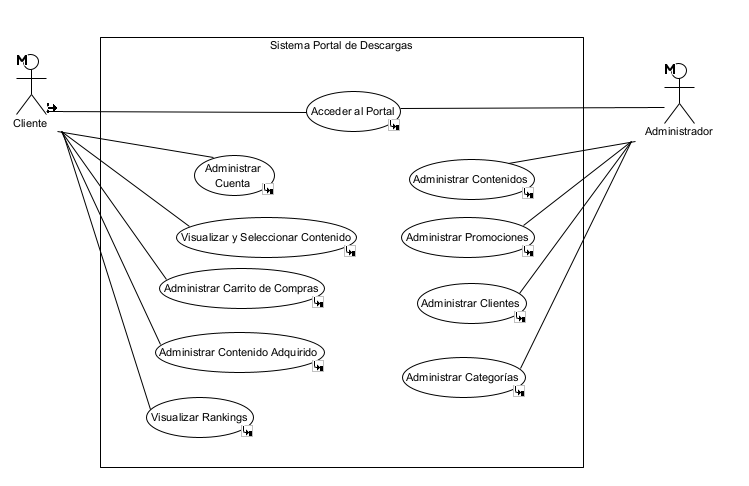
\includegraphics[width=0.9\textwidth]{Media/3_Analisis/3_ModeloDeRequisitos/CasosDeUso.png}
    \caption{Diagrama de casos de uso} 
    \label{fig:DiaramaCasoDeUso}
\end{figure}

\textbf{Archivo:} Diagrama de Casos de Uso (formato Visual Paradigm) \\
\textbf{Link de descarga:} \linkDiagramaCasoDeUso \\

\textbf{Pasos de ejecución:}
\begin{itemize}
    \item Ingresar al repositorio en GitHub usando el link proporcionado y descargar el archivo QCM.vpp
    \item Abrir el archivo descargado en la herramienta Visual Paradigm.
    \item En la pestaña Diagram Navigator abrir UML Diagrams
    \item Abrir Use Case Diagram y seleccionar Diagrama de Casos de Uso QCM.

\end{itemize}

\newpage
\subsubsection{Especificación de Casos de uso}
Se detallan las especificaciones de cada caso de uso del diagrama de casos de uso de la figura~\ref{fig:DiaramaCasoDeUso}. La Tabla \ref{tab:especCU} muestra la especificación correspondiente al caso de uso CU-001: Acceder al portal.

%%%%%%%%%%%%%%%%%%%%%%%%%%%%%% Configuración de tabla
\renewcommand{\arraystretch}{1.5}
\begin{longtable}{|p{15cm}|}
\caption{Especificación del caso de uso CU-001: Acceder al portal}
\label{tab:especCU}\\
\hline
\endfirsthead

\multicolumn{1}{c}%
{{\bfseries \tablename\ \thetable{} -- continuación desde la página anterior}} \\
\hline
\endhead

\hline \multicolumn{1}{r}{{Continúa en la siguiente página}} \\
\endfoot

\hline
\endlastfoot
%%%%%%%%%%%%%%%%%%%%%%%%%%%%%%

\textbf{Caso de uso:} Acceder al portal \\
\hline
\textbf{ID:} CU-001 \\
\textbf{Descripción:} El sistema permite a los usuarios autenticarse o registrarse en el sistema ingresando su username y contraseña. Dependiendo del tipo de usuario, se redirige al cliente (OBJ-001) al portal de venta de contenido o al administrador (OBJ-002) al portal de administración del sistema. \\
\hline

\textbf{Actores principales:}
\begin{itemize}
    \item Cliente
    \item Administrador
\end{itemize} \\
\hline

\textbf{Precondiciones:} \\
Ninguna \\
\hline

\textbf{Flujo principal:}
\begin{itemize}
\item Al ingresar a la página de QuickContentMedia lo primero que se mostrará es la UIAccesoAlPortal (MK-001) donde el usuario tendrá disponibles las opciones Log In o Sign Up según sea cliente (OBJ-001) o administrador (OBJ-002):
  \begin{itemize}
  \item \textbf{Log In (cliente y administrador): }En la UIAccesoAlPortal (MK-001), el usuario deberá completar los cuadros de texto de username y contraseña, y luego hacer clic en el botón “Log in”. La UIAccesoAlPortal (MK-001) envía las credenciales a gestorUsuario (G-001), que verifica que correspondan a un cliente (OBJ-001) activo en la tabla Clientes (BD-001) o a un administrador (OBJ-002) en la tabla Administradores (BD-002). Si la autenticación es válida, la UIAccesoAlPortal (MK-001) redirige al usuario a la UIInicioCliente (MK-003) o a la UIInicioAdmin (MK-024), según sea cliente (OBJ-001) o administrador (OBJ-002) correspondientemente.

  \item \textbf{Sign Up (solo cliente):} En la UIAccesoAlPortal (MK-001), el cliente (OBJ-001) selecciona la opción “Registrarse”. La UIAccesoAlPortal (MK-001) lo redirige a la UIRegistroCliente (MK-002), donde deberá ingresar su nombre, apellido, username y contraseña, y luego hacer clic en el botón “Sign up”. La UIRegistroCliente (MK-002) envía la información a gestorUsuario (G-001), que verifica que el username no esté asociado a un cliente (OBJ-001) existente en la tabla Clientes (BD-001). Si el username no se encuentra registrado, gestorUsuario (G-001) almacena los datos del nuevo cliente (OBJ-001) en la tabla Clientes (BD-001) y la UIRegistroCliente (MK-002) lo redirige a la UIInicioCliente (MK-003).
  \end{itemize}
\end{itemize} \\
\hline

\textbf{Flujo alternativo:}
\begin{itemize}
\item Si el username ingresado por el cliente (OBJ-001) en la UIRegistroCliente (MK-002) ya está asociado a una cuenta existente, el sistema mostrará la UIErrorRegistro (MK-048) con el botón “Continuar” que redirige al cliente (OBJ-001) a la UIRegistroCliente (MK-002) para que pueda corregir el dato.

\item Si las credenciales proporcionadas por el usuario en la UIAccesoAlPortal (MK-001) no son válidas, el sistema mostrará la UIErrorLogin (MK-040) indicando que el username o la contraseña son incorrectos. Esta interfaz incluye un botón “Volver”, el cual redirige nuevamente a la UIAccesoAlPortal (MK-001).
\end{itemize} \\
\hline

\textbf{Postcondiciones:}
\begin{itemize}
\item El usuario ha iniciado sesión correctamente y es redirigido al portal correspondiente según su rol (cliente o administrador).
\item En caso de que un cliente (OBJ-001) se haya registrado, sus credenciales han sido almacenadas en la tabla Clientes (BD-001).
\end{itemize} \\
\hline

\end{longtable}
%%%%%%%%%%%%%%%%%%%%%%%%%%%%%% Fin de tabla
\textbf{Documento:} Especificaciones de Casos de Uso \\
\textbf{Link de acceso:} \linkDiagramaEspecificacionesCasoDeUso \\

